\section*{3. Расчет каскада методом AC и гармонического баланса (Harmonic Balance)}

В данном разделе проводится анализ нелинейной модели транзистора в одной рабочей точке при воздействии малого сигнала (метод AC). Для расчета используется схема с питанием от одного источника постоянного напряжения ($V_C = 2.5$ В), где необходимое смещение на базу задается с помощью резистивного делителя, состоящего из сопротивлений $R_{35}$ и $R_{36}$. На вход каскада (порт 1) подается высокочастотный сигнал, а выход нагружен на стандартное сопротивление 50 Ом.

\begin{figure}[H]
	\centering
	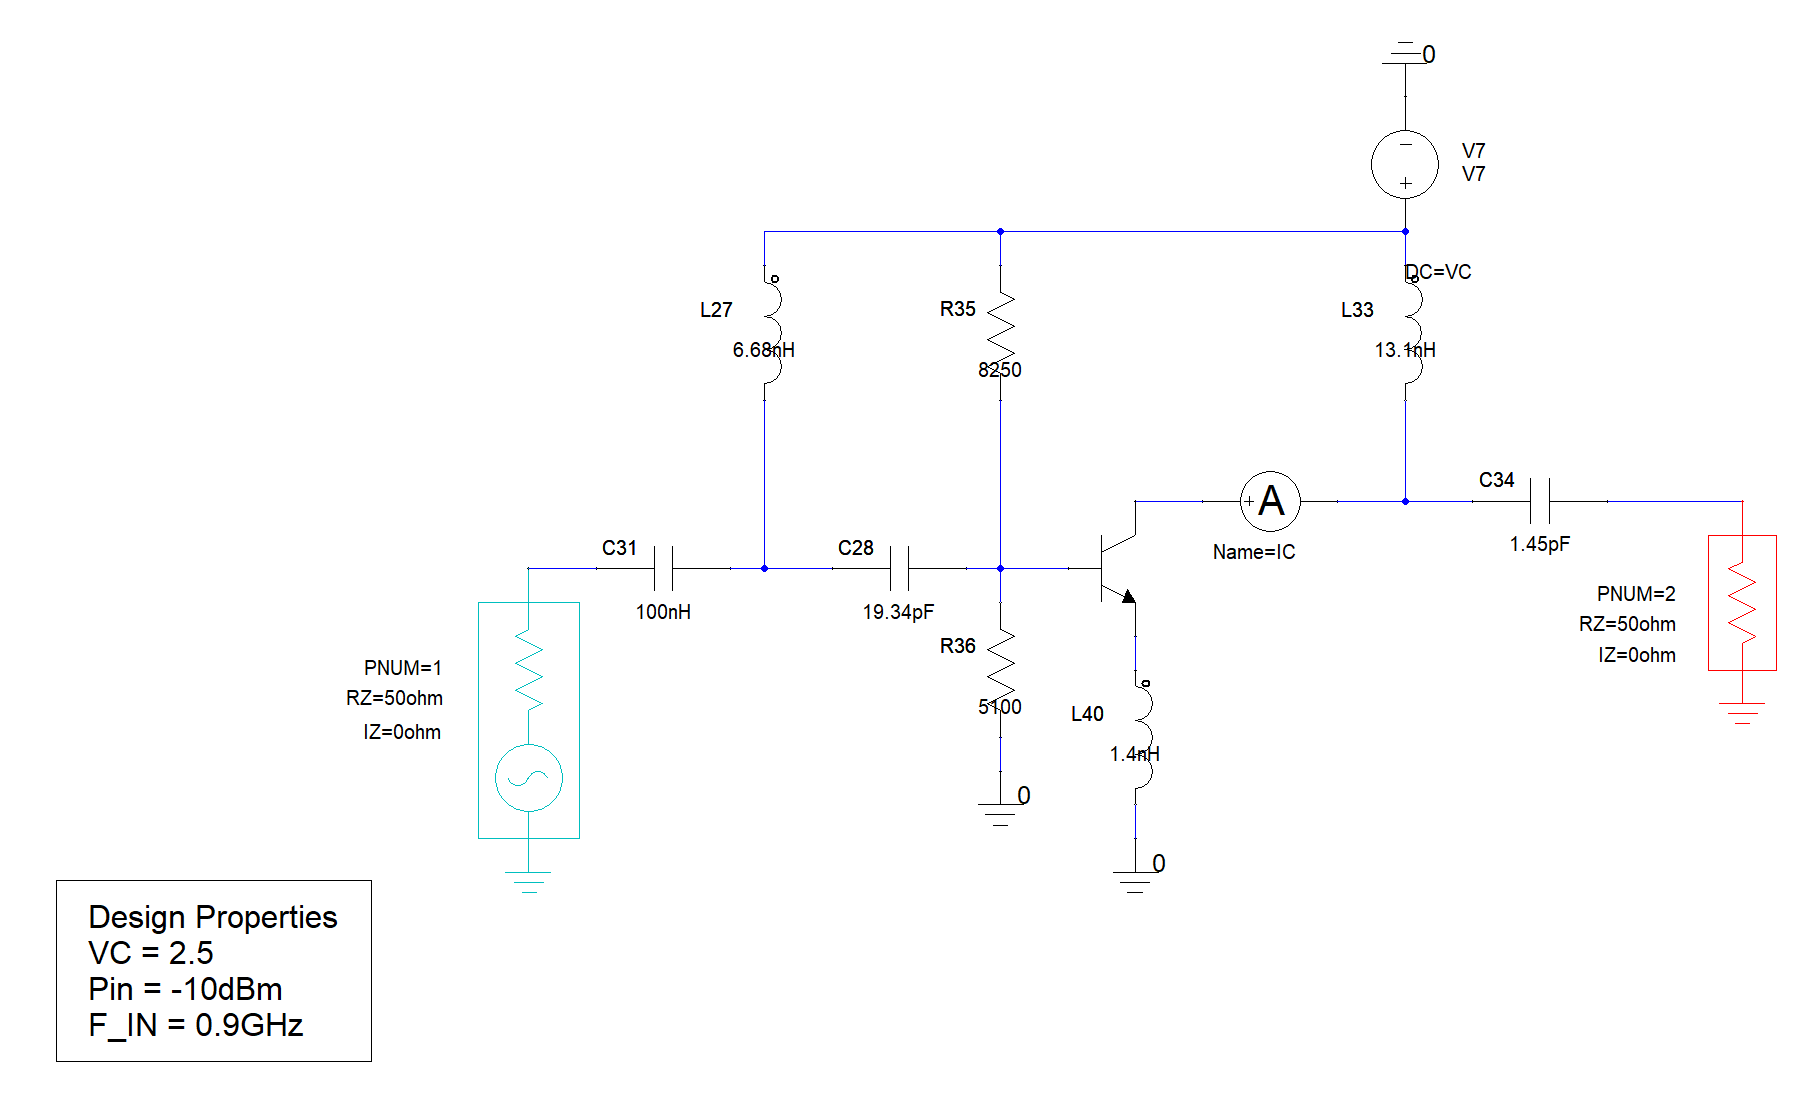
\includegraphics[width=0.8\textwidth]{12.PNG}
	\caption{Схема усилителя на транзисторе NE68133 с питанием от источника DC и резистивным делителем напряжения.}
	\label{fig:ac_schema}
\end{figure}

Расчет малосигнальных частотных характеристик выполняется с помощью инструмента \verb|Linear Network Analysis| в частотной области. В настройках анализа задается диапазон развертки частоты (от 2 до 3 ГГц с шагом 0.01 ГГц) и включается опция расчета шума (\verb|Enable Noise Calculation|). 

\begin{figure}[H]
	\centering
	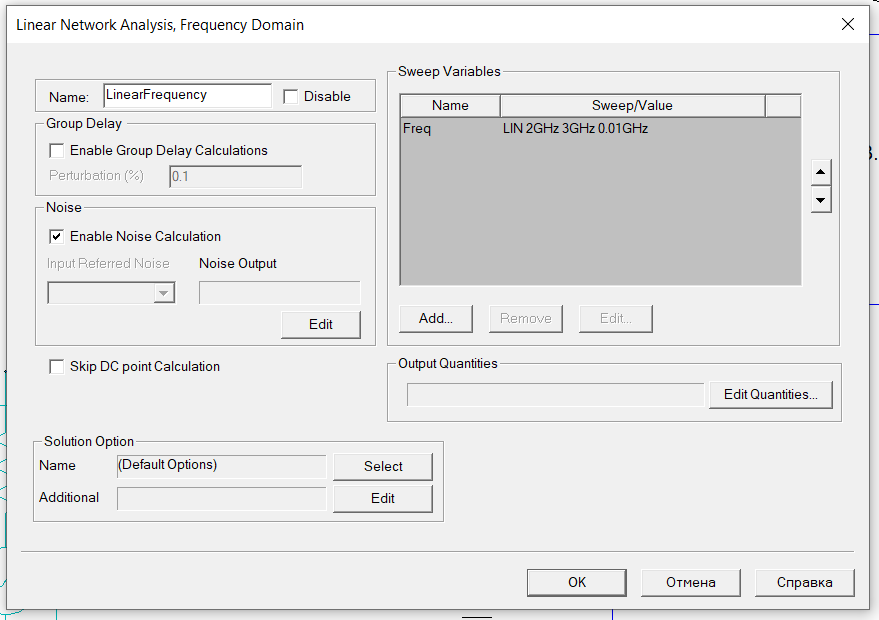
\includegraphics[width=0.7\textwidth]{13.PNG}
	\caption{Настройки линейного частотного анализа (Linear Network Analysis) с расчетом шума.}
	\label{fig:ac_setup}
\end{figure}

По результатам линейного анализа строятся графики зависимости коэффициентов отражения ($S_{11}$, $S_{22}$), коэффициента передачи ($S_{21}$) и коэффициента шума (NF) от частоты. Данный метод позволяет получить малосигнальные характеристики каскада, учитывающие свойства нелинейной модели транзистора в заданной рабочей точке по постоянному току.

\begin{figure}[H]
	\centering
	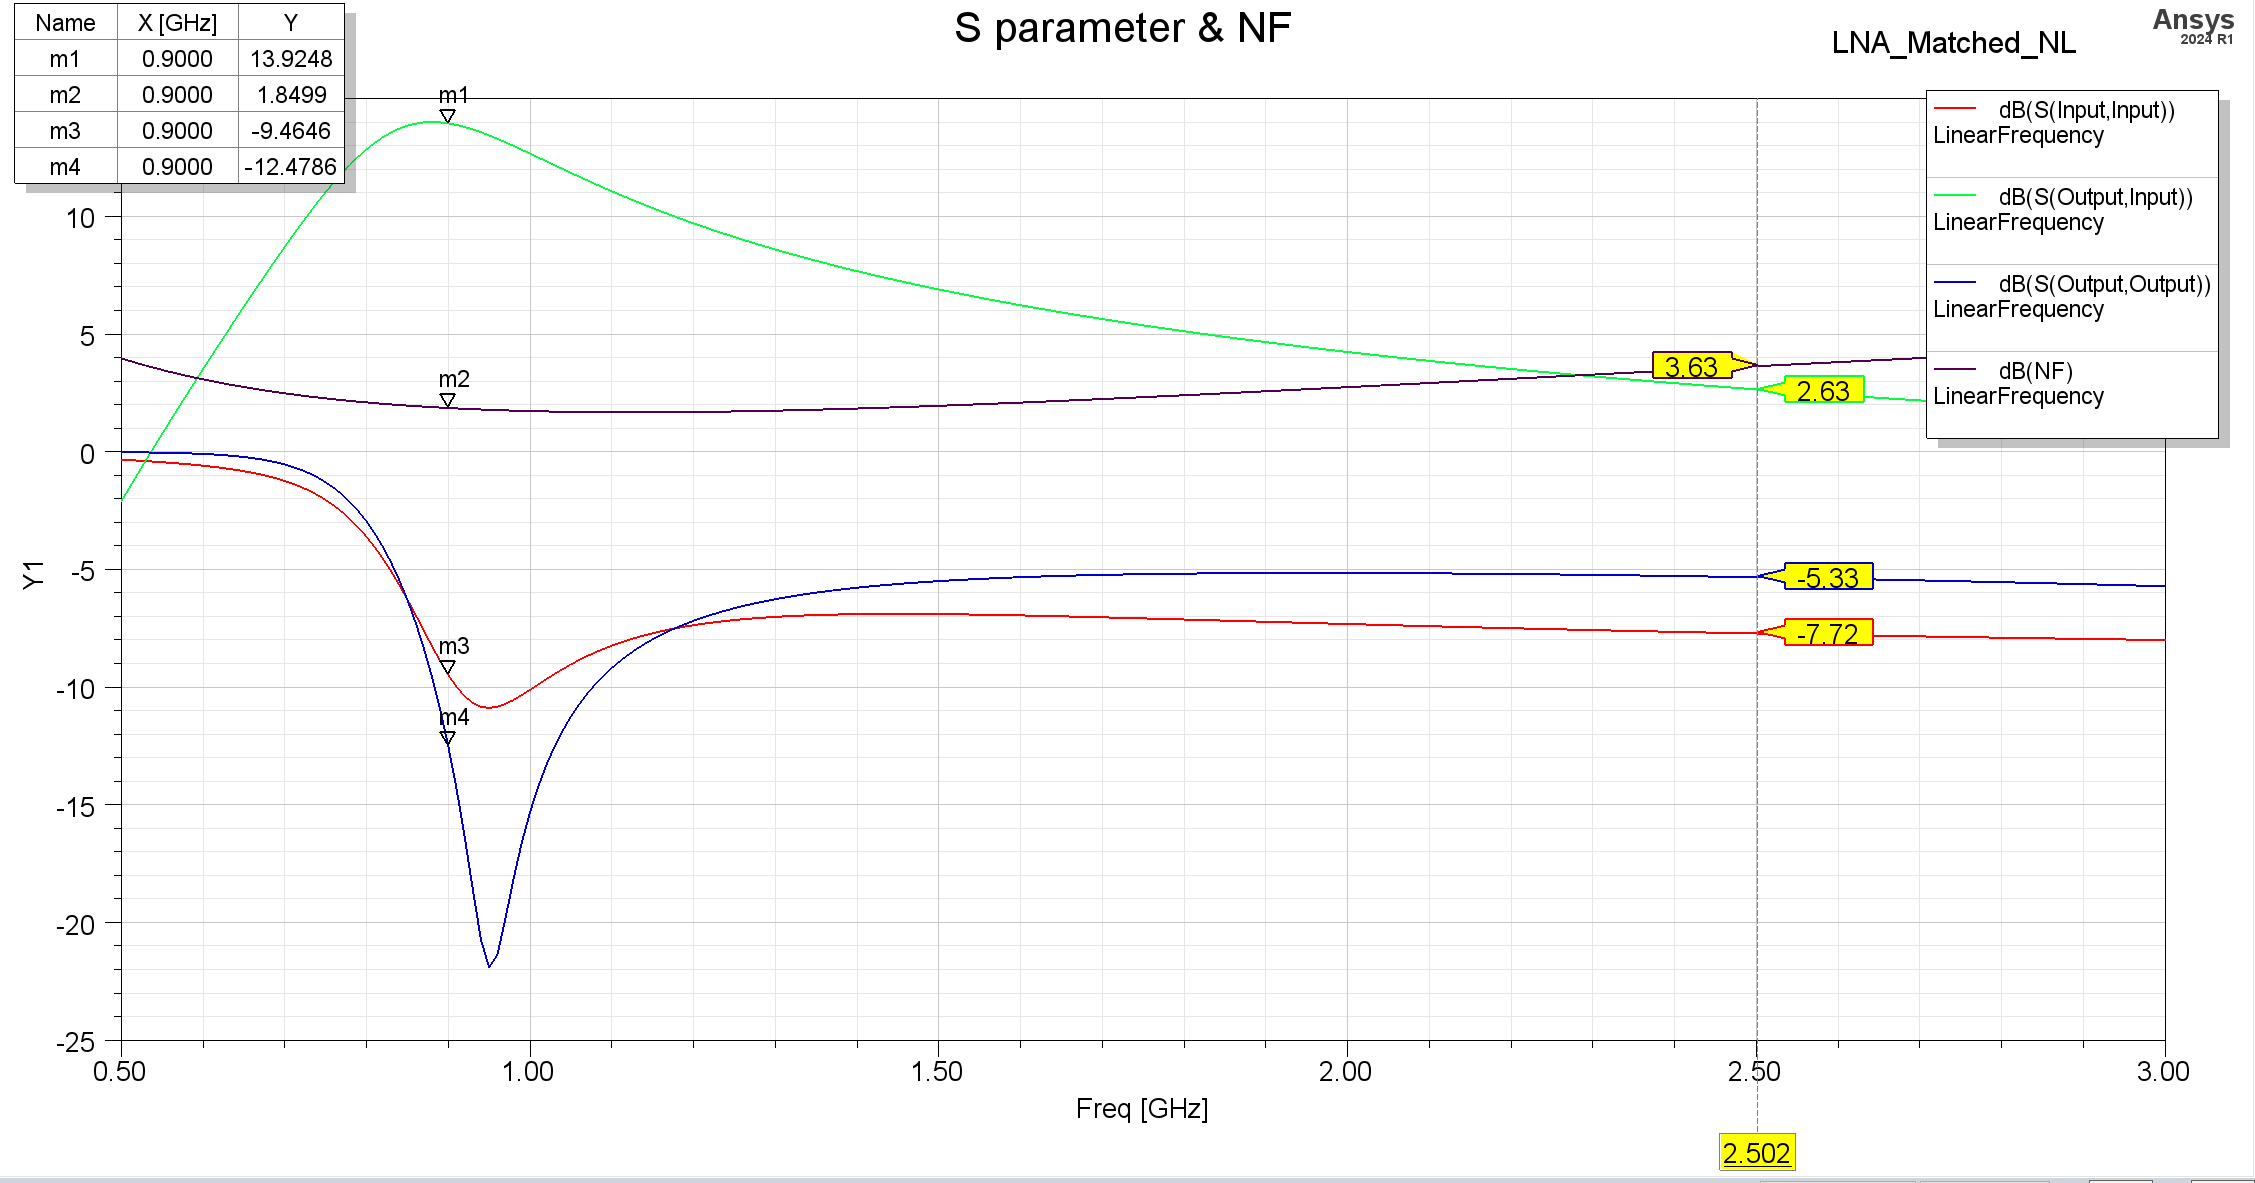
\includegraphics[width=0.9\textwidth]{14.PNG}
	\caption{Линейные характеристики каскада: S-параметры и коэффициент шума (NF).}
	\label{fig:ac_results}
\end{figure}

Для оценки нелинейных искажений усилителя, в частности компрессии усиления, применяется метод гармонического баланса (Harmonic Balance 1-Tone). В диалоговом окне настроек устанавливается расчет до 7-й гармоники, а мощность входного сигнала (\verb|Pin|) задается в виде развертки в диапазоне от -40 дБм до 10 дБм с шагом 1 дБм.

\begin{figure}[H]
	\centering
	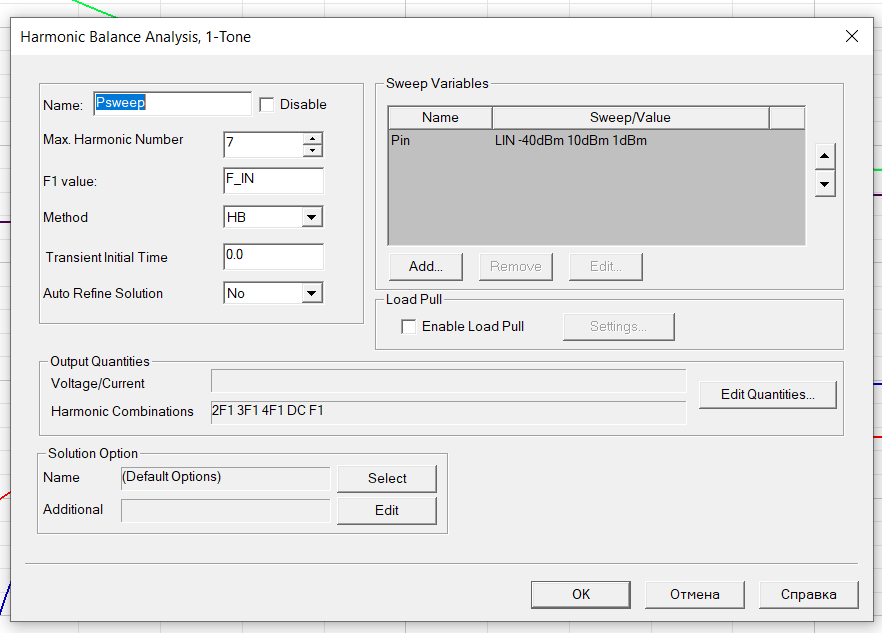
\includegraphics[width=0.7\textwidth]{15.PNG}
	\caption{Задание параметров расчета методом однотонового гармонического баланса.}
	\label{fig:hb_setup}
\end{figure}

Результаты нелинейного анализа представляются в виде зависимостей выходной мощности на основной частоте (\verb|Pout@Fundamental|) и коэффициента передачи (\verb|TG21@Fundamental|) от уровня входной мощности \verb|Pin|. По полученному графику определяется точка децибельной компрессии (P1dB) — уровень, при котором коэффициент усиления снижается на 1 дБ относительно своего линейного малосигнального значения. На графике видно, что при входной мощности -40 дБм коэффициент передачи составляет 13.92 дБ (маркер m1), а падение усиления на 1 дБ (до 12.88 дБ, маркер m2) происходит при входной мощности -8 дБм, что определяет верхнюю границу динамического диапазона данного усилителя.

\begin{figure}[H]
	\centering
	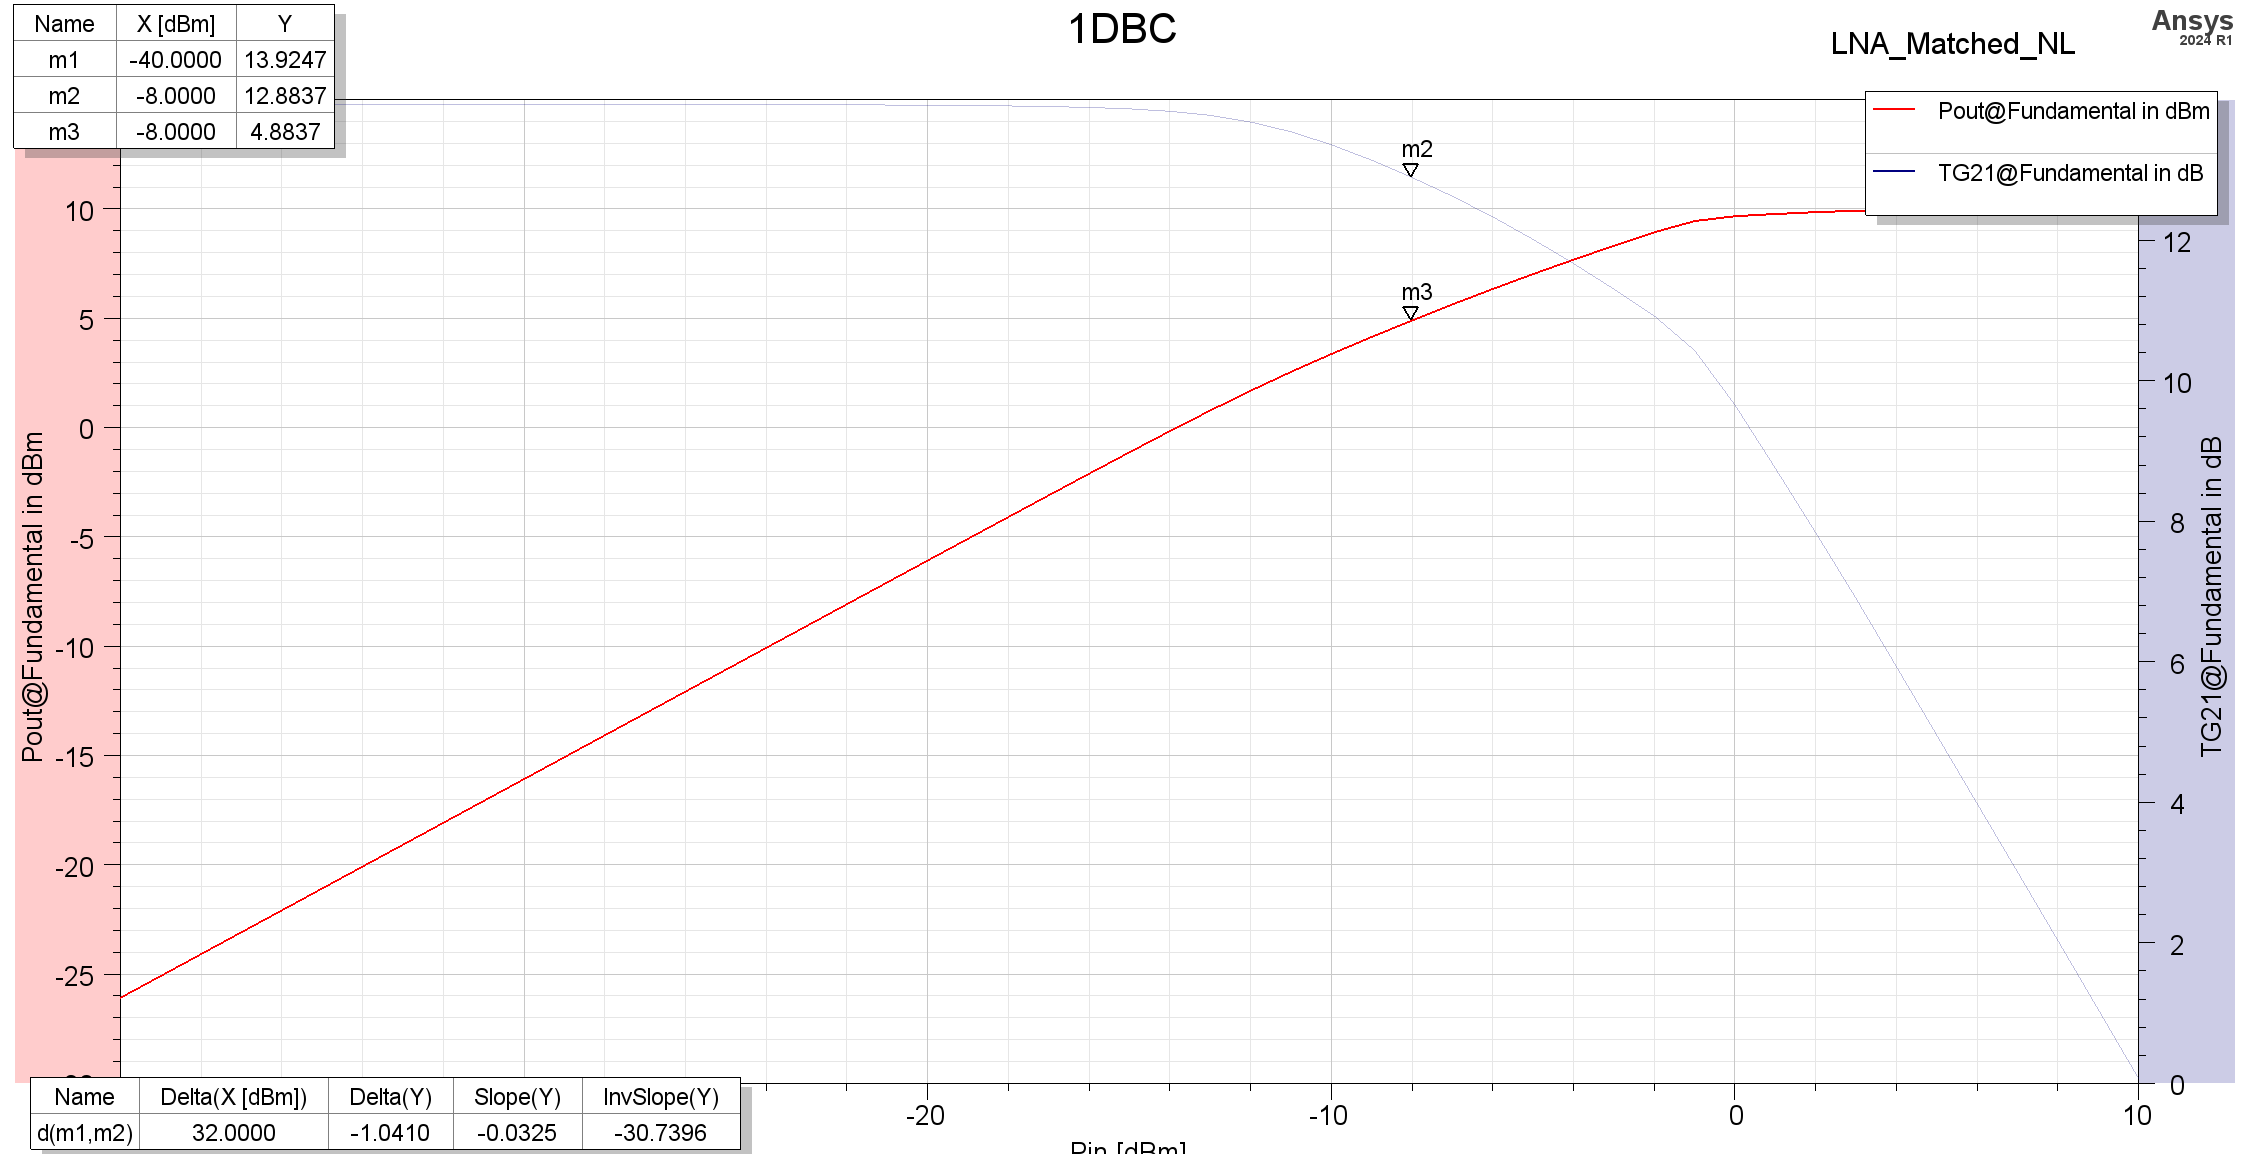
\includegraphics[width=0.9\textwidth]{16.PNG}
	\caption{Нелинейные зависимости выходной мощности и коэффициента передачи от входной мощности (точка компрессии 1 дБ).}
	\label{fig:hb_compression}
\end{figure}